\documentclass[3p]{elsarticle}
%\documentclass[3p, twocolumn]{elsearticle}
\usepackage{amsmath}
\usepackage{amssymb}
\usepackage{gensymb}
\usepackage{upgreek}
\usepackage{float}
\parskip=0pt

\begin{document}

\begin{frontmatter}

\title{Novel cat's--whisker electrode for \emph{in-situ} corrosion product monitoring}
\cortext[cor]{Corresponding author}
\author[akiss]{Andr\'{a}s Kiss\corref{cor}}
\address[akiss, gnagy]{Department of General and Physical Chemistry, Faculty of Sciences, University of P\'{e}cs, 7624 P\'{e}cs, Ifj\'{u}s\'{a}g \'{u}tja 6, Hungary}
\address[akiss, gnagy]{J\'{a}nos Szent\'{a}gothai Research Centre, University of P\'{e}cs, 7624 P\'{e}cs, Ifj\'{u}s\'{a}g \'{u}tja 20, Hungary}
\ead{akiss@gamma.ttk.pte.hu}
\author[gnagy]{G\'{e}za Nagy}
\ead{g-nagy@gamma.ttk.pte.hu}

\begin{abstract}
\end{abstract}

\begin{keyword}
	scanning electrochemical microscope \sep corrosion product
\end{keyword}
\end{frontmatter}

\begin{figure}[H]
\centering
% trim = top left bottom right
\includegraphics[trim = 20mm 30mm 0mm 20mm, clip, width=0.3\textwidth, angle=-90]{17052401.eps} 
\includegraphics[trim = 20mm 30mm 0mm 20mm, clip, width=0.3\textwidth, angle=-90]{17052402.eps}
\includegraphics[trim = 20mm 30mm 0mm 20mm, clip, width=0.3\textwidth, angle=-90]{17052403.eps} 
\includegraphics[trim = 20mm 30mm 0mm 20mm, clip, width=0.3\textwidth, angle=-90]{17052405.eps}
\includegraphics[trim = 20mm 30mm 0mm 20mm, clip, width=0.3\textwidth, angle=-90]{18011710.eps} 

% trim = left bottom right top
%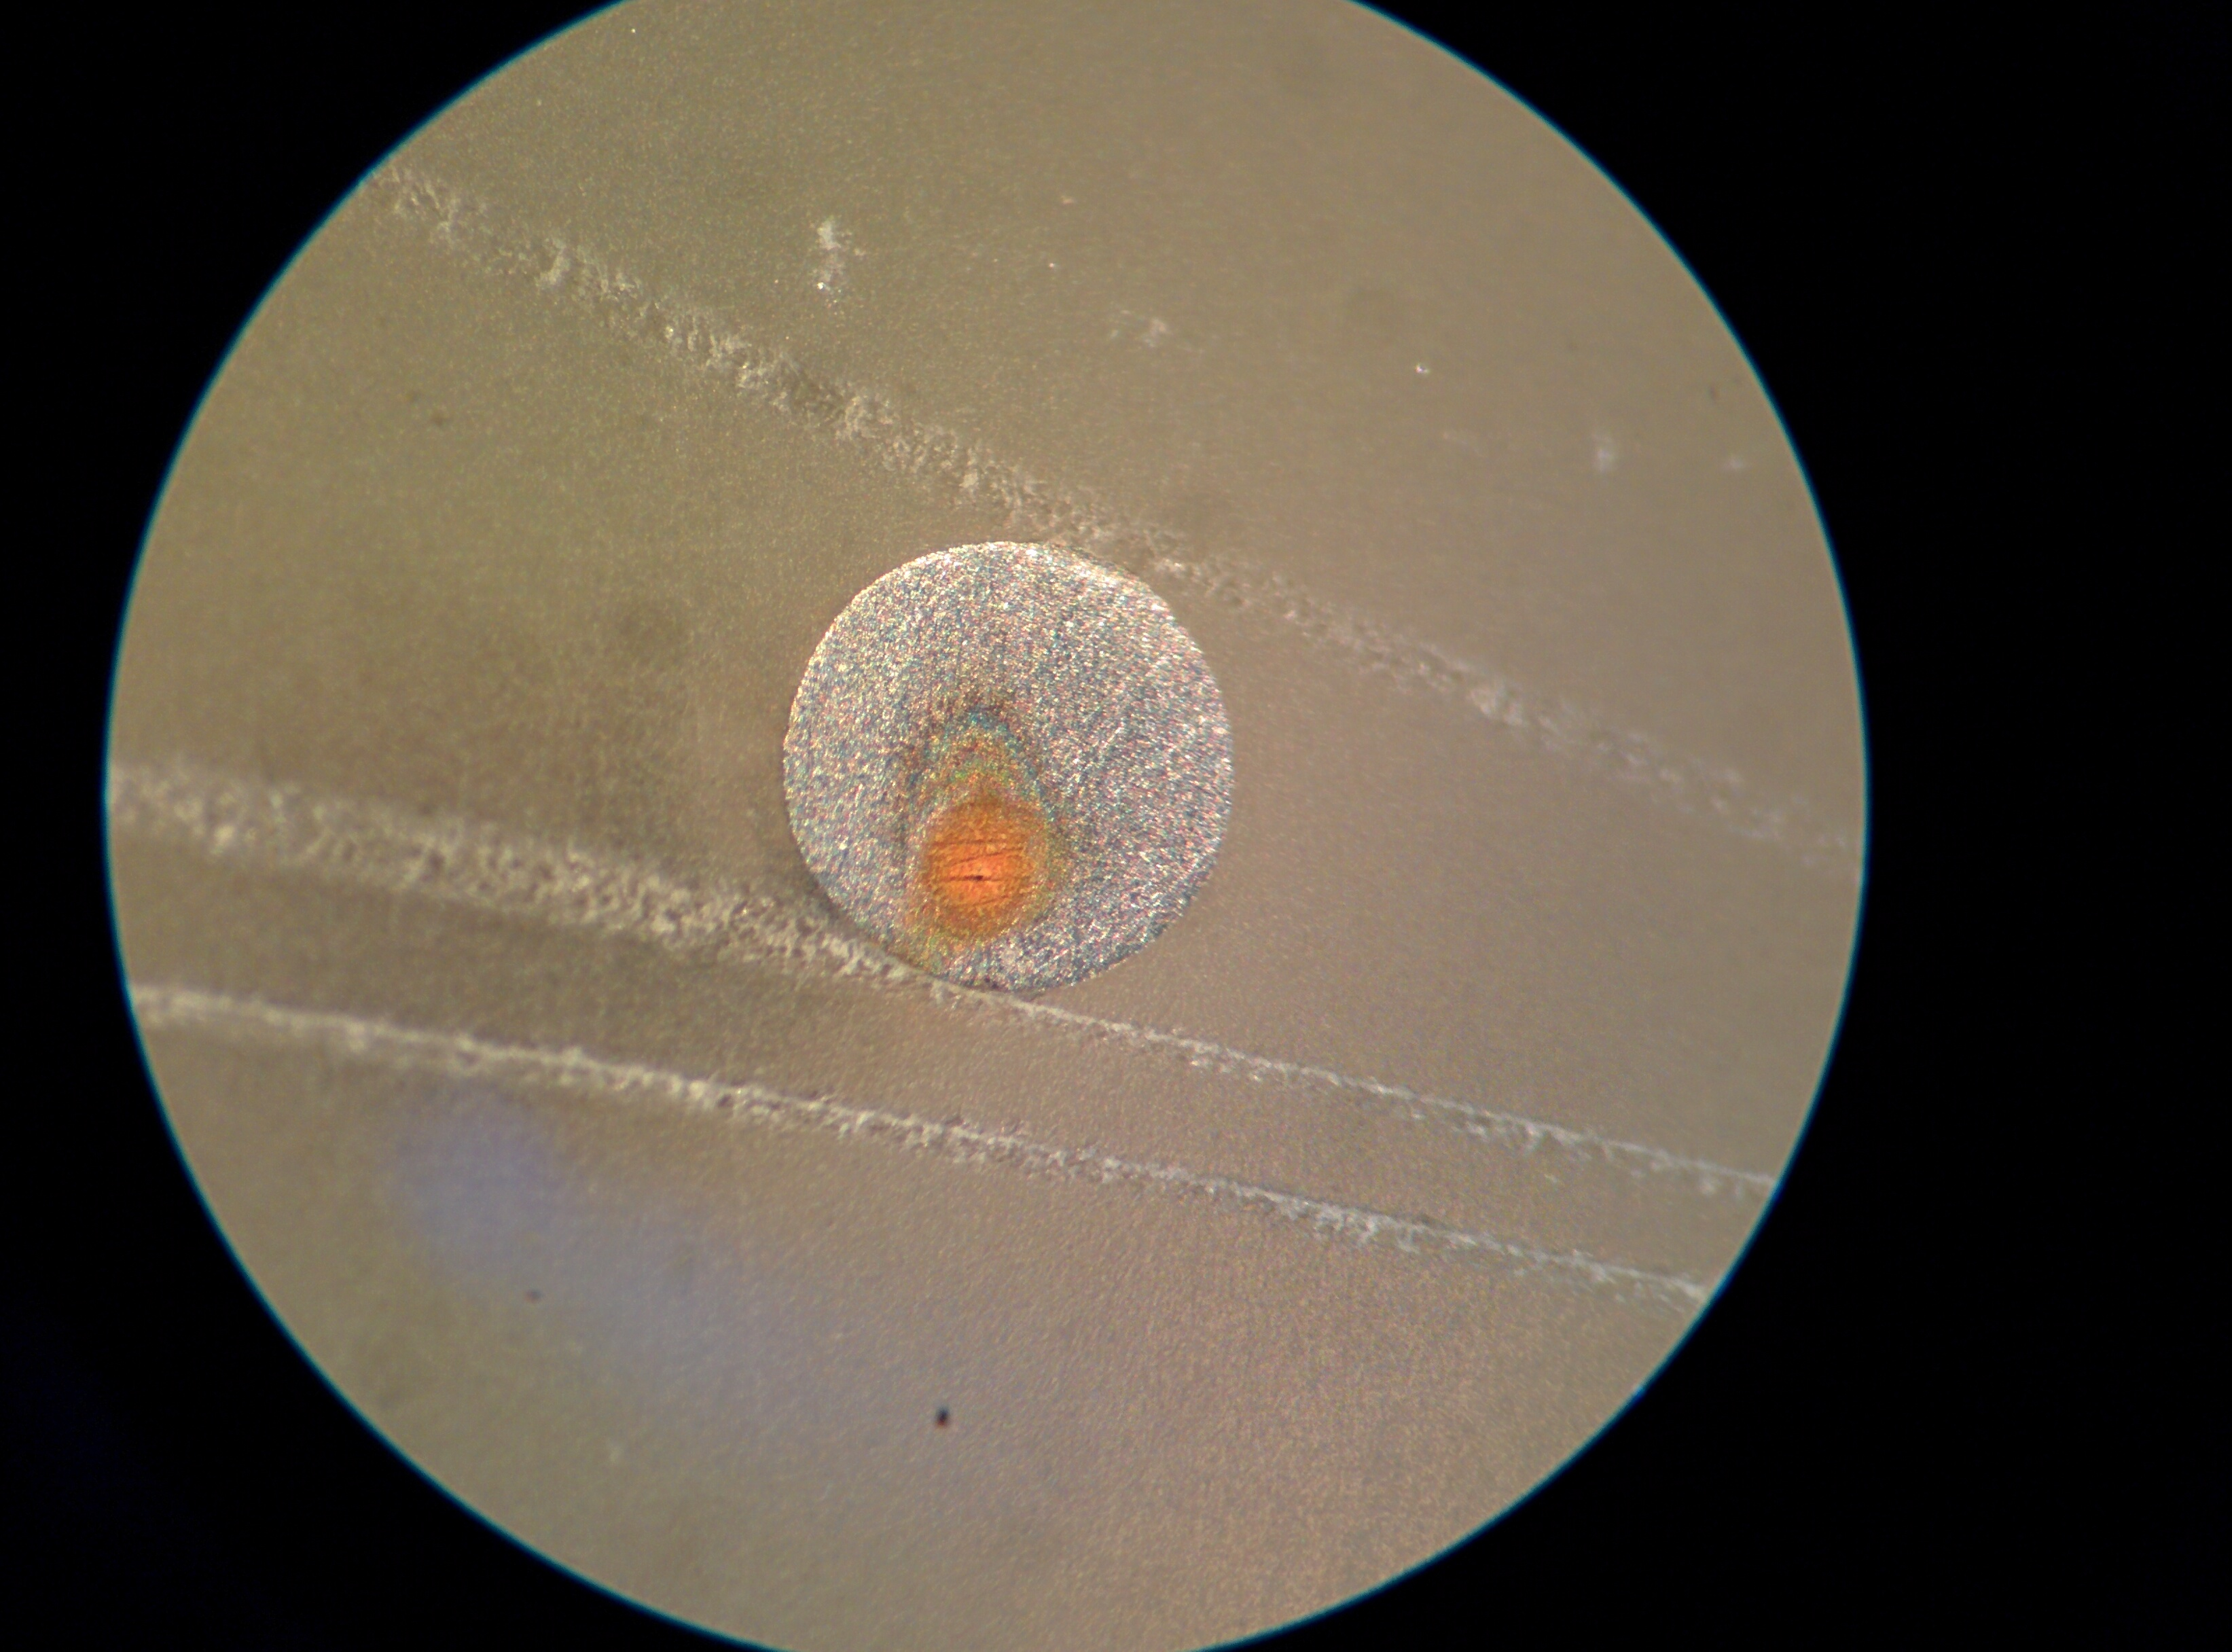
\includegraphics[trim = 350mm 300mm 460mm 250mm, clip, width=0.25\textwidth]{IMG.jpg}
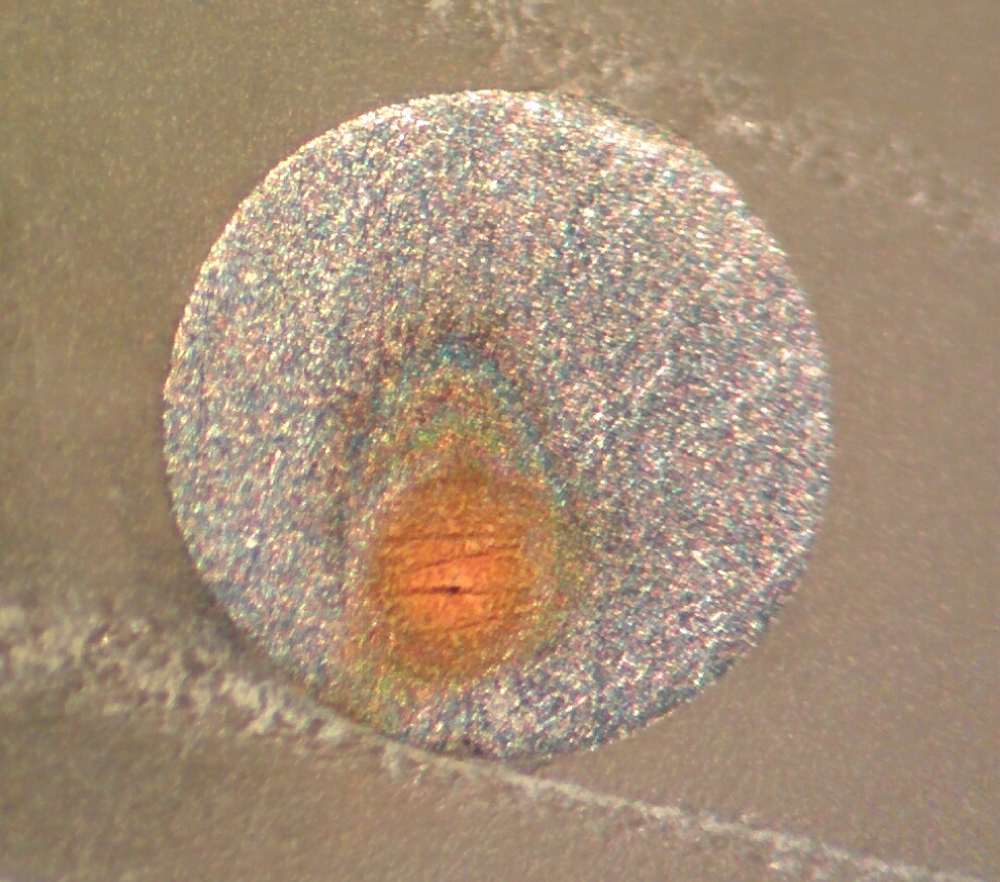
\includegraphics[width=0.25\textwidth]{img1.png}
\hspace{2cm}
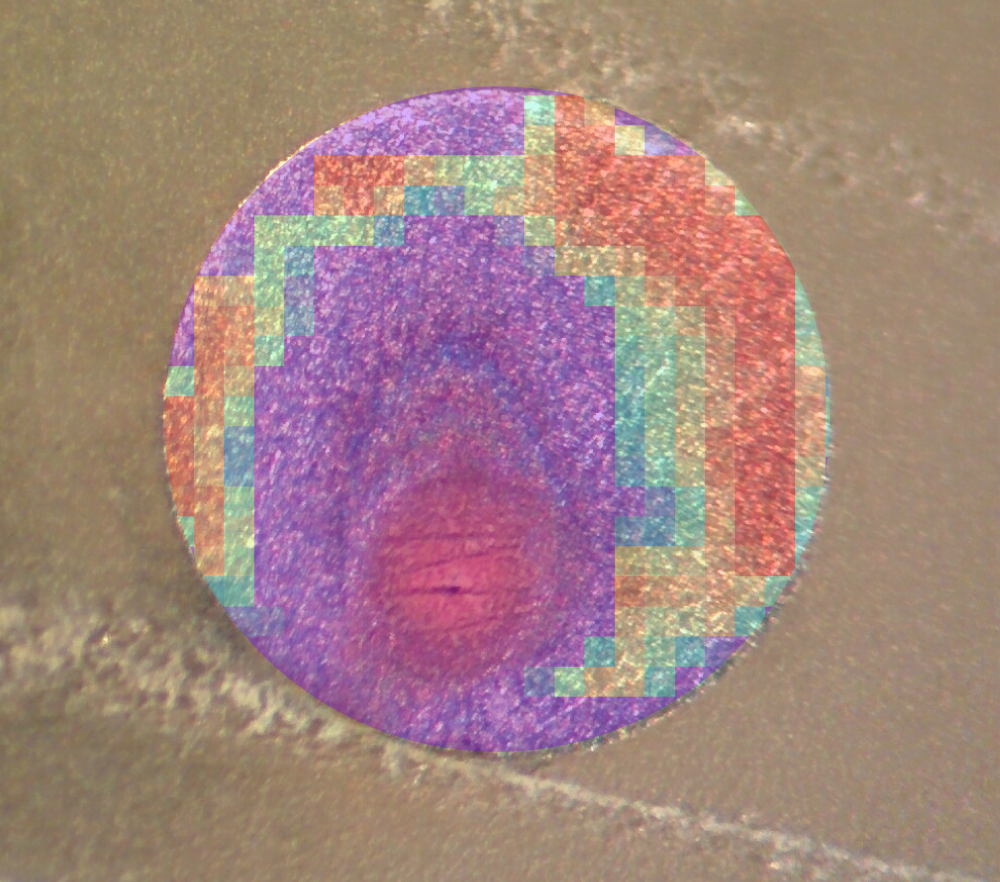
\includegraphics[width=0.25\textwidth]{img2.png}

\caption{Figure caption.}
\label{fig:deconvolution}
\end{figure}

\begin{figure}[H]
\centering
% trim = top left bottom right
% trim = left bottom right top
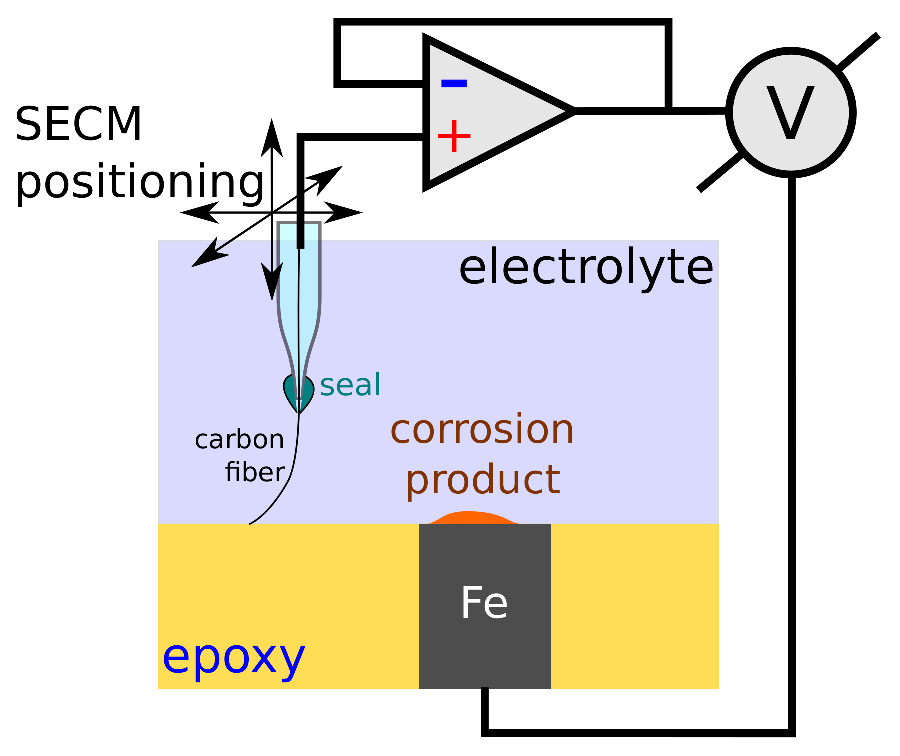
\includegraphics[width=0.6\textwidth]{whisker.eps}
%\includegraphics[trim = 20mm 30mm 0mm 20mm, clip, width=0.3\textwidth, angle=-90]{13121223.eps} 
\caption{Figure caption.}
\label{fig:deconvolution}
\end{figure}


\end{document}
